% !TEX encoding = UTF-8 Unicode
\documentclass[12pt]{article}
\usepackage{geometry}
\geometry{a4paper}
\usepackage[utf8]{inputenc}
\usepackage{enumerate}
\usepackage{array}
\usepackage{fancyhdr}
\usepackage{parskip}
\usepackage{xlop}
\usepackage{color}
\usepackage{graphicx}
\usepackage[colorlinks=true, urlcolor=blue, linkcolor=black]{hyperref}
\usepackage[T1]{fontenc}
\usepackage{listings}
\usepackage[colorinlistoftodos,prependcaption,textsize=tiny]{todonotes}

\renewcommand{\arraystretch}{1.5}
\newcolumntype{B}{>{\bfseries}c}
\setlength{\parsep}{\parskip}

%----------------------------------------------------------------------------------------
%	TITLE PAGE
%----------------------------------------------------------------------------------------

\newcommand{\titleAT}{\begingroup % Create the command for including the title page in the document
\newlength{\drop} % Command for generating a specific amount of whitespace
\drop=0.07\textheight % Define the command as 10% of the total text height

\rule{\textwidth}{1pt}\par % Thick horizontal line
\vspace{2pt}\vspace{-\baselineskip} % Whitespace between lines
\rule{\textwidth}{0.4pt}\par % Thin horizontal line

\vspace{\drop} % Whitespace between the top lines and title
\centering % Center all text

{\Huge CockpitVR - Group 6}\\ % Title

\vspace{\drop} % Whitespace between the title and short horizontal line
\rule{0.3\textwidth}{0.4pt}\par % Short horizontal line under the title
\vspace{\drop} % Whitespace between the thin horizontal line and the author name

\bigskip

{\large \textsc{Adan Häfliger, Jonathan Link \& Xavier Willemin}}\par % Author name
{\Small Supervised by Prof. Ronan Boulic \& Thibault Porssut}\par % Author name

\bigskip
\bigskip

{\small \textsc{26 mai 2017}}\par % Date

\vfill % Whitespace

\begin{figure}[!h]
	\centering
	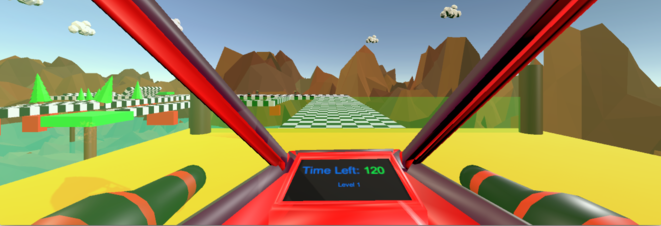
\includegraphics[scale=1.25]{images/cover.png}
\end{figure}

\bigskip
\bigskip
\bigskip
\bigskip

\rule{\textwidth}{0.4pt}\par % Thin horizontal line
\vspace{2pt}\vspace{-\baselineskip} % Whitespace between lines
\rule{\textwidth}{1pt}\par % Thick horizontal line

\thispagestyle{empty}

\endgroup}

%----------------------------------------------------------------------------------------
%	END TITLE PAGE
%----------------------------------------------------------------------------------------

\begin{document}

\titleAT

\newpage

\tableofcontents

\newpage

CockpitVR is a game initially inspired from Gundam. You are immersed in the cockpit of a robot equipped with one canon in each hand and move in the level. The goal is to reach one of the green platforms in a given amount of time. Of course, some obstacles prevent you from progressing too fast : walls, turrets, moving floors.

Since gaming is better when experienced in multiplayer, we also implemented an asymmetric gameplay that can be scaled to any number of players. There roles is to activate the obstacles slowing the progression of the Vive-equipped player by triggering obstacles at distance through a tablet.

\section{Game design \& rules}

Since no blood is allowed in this project, we opted for a time-oriented approach. This means that you cannot die in our game. You can just run out of time. If the user falls of the pathway, the robot is teleported at the beginning of the level. Of course, the time continues to elapse and is not reset. So be quick, but be careful not to fall to avoid losing too much time by starting over !

You can control the robot the following way :

\begin{itemize}
	\item Pitch one or both controllers forward to move forward and backward to move backwards
	\item Yaw one or both controllers to move sideways
	\item Roll one or both controllers to rotate on yourself
\end{itemize}

You can of course combine any of these three basic controls to move more freely.

When both controllers are used to move the robot, the average of both inputs is computed. This has the benefit to increase the precision of the movement of the robot with respect to your hands. To disengage a controller, hold its trigger button (below your index). You will then move the canon of the corresponding hand.

At the moment, the following features and interactions are available in the first level :

\begin{itemize}
	\item Shrinking pathway along the course to force the mastering of the movement metaphor.
	\item Rotating blocs of pathway, requiring the user to carefully time its movements to avoid falling.
	\item Walls that appear for predetermined duration that the user can avoid. Be careful, some of these walls might surprise and/or frighten you, as they are tagged with images (Trump faces, for instance).
	\item Destroyable walls (distinguished from the other walls by a painted target-sign). The user needs to shoot the wall multiple times with his canons to destroy it.
	\item Turrets projecting flames. The flames will not hurt you, but rather strongly unbalance your robot. You should then avoid them if you do not want to fall.
\end{itemize}

These obstacles can be triggered by other players connected to the host (the computer to which the Vive is connected) with their device (tablet, smartphone or computer). They will see a scrollable 2D view of the level from above, called the minimap (see figure below). This map is refreshed every second to display the position of the robot. A latency in the refresh rate has been added to increase the difficulty.

The minimap also shows the position of the obstacles that can be triggered by the network players. Clicking on them activates the obstacle.

\begin{figure}[h]
   \caption{\label{étiquette} The players of the minimap can trigger the obstacles over the Internet.}
   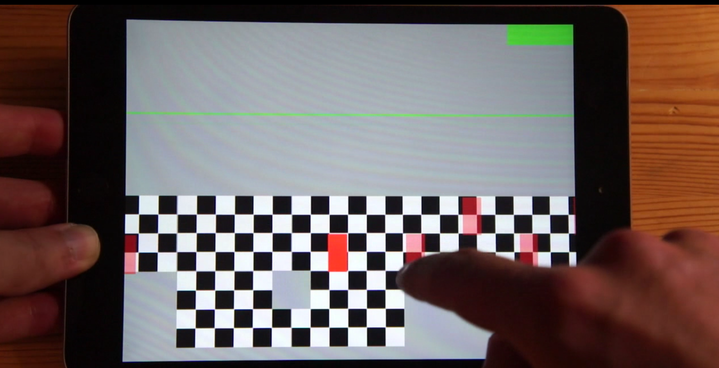
\includegraphics[scale=0.8]{images/minimap.png}
\end{figure}

\section{Running the project}

\subsection{Technical requirements}

As for any virtual reality project, both the hardware and software requirements can't be neglected. We can guarantee that the project is running in the following configuration, but might as well in different environments :

\begin{itemize}
	\item HTC Vive in a calibrated room-scale (2 lighthouses, 1 HMD and 2 controllers)
	\item A powerful computer with a gaming graphic card (tested with an Nvidia GTX Titan). Check \href{https://www.vive.com/us/ready/}{www.vive.com/us/ready} for more informations.
	\item Unity 5.5+ (tested on 5.5.2)
	\item SteamVR with a Steam account
	\item Any tablet, smartphone or computer (for the players without the Vive in multiplayer)
\end{itemize}

\subsection{Setup}

\begin{enumerate}
	\item Turn on the lighthouses and wait that they sync each other.
	\item Turn on the HMD and the two controllers and check that they are tracked.
	\item Place a chair in the tracking area and sit on it once you wear the HMD and have the controllers in your hands.
	\item Launch the .exe file (or ask somebody to do it for you). Note that the game will be oriented with respect to the orientation of the HMD at the moment of the launch.
	\item Since you will use the 3D orientation of the controllers to move the robot and its arms, you now have to calibrate the neutral orientation of the controllers. So relax and once you are in a comfortable position, stay more or less steady with your hands and click on one of the grip buttons (the rounded-rectangles on the handle under your palm) of one of the controllers. This step will also reliably compute which controller is in your left hand and which one is in your right one.
	\item You are now ready to play ! You can take your time at this point in the yellow zone, but be careful ; once you are on the checkered-flag pathway the time starts ticking... (see figure below)
\end{enumerate}

\begin{figure}[!h]
   \caption{\label{étiquette} Top view of the level}
   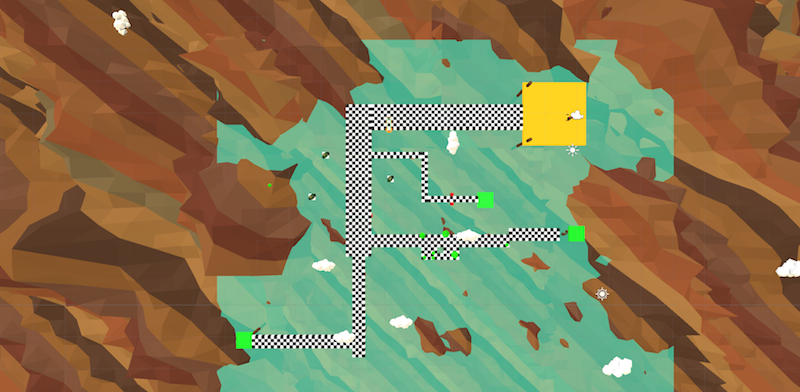
\includegraphics[scale=0.53]{images/topview.png}
\end{figure}

Hint : if you do not want to move the robot but still need to move your hands, you can hold the trigger of both controllers. This will indeed disengage the controllers as a way to move the robot and move the canons instead.

\section{Implementation}

\subsection{HTC Vive Interaction}

Since this is a VR project, we worked a lot to build a convincing experience for the user with the help of the VR hardware, namely the HTC Vive. We also wanted to be innovative and bring to the field new means of interaction between the player and the virtual game. That is why we developed an algorithm to be able to use the Vive controllers as a joystick, which is to us the most user-friendly way of driving without any additional (and costly) hardware. Here are the details of its implementation.

We first captured the orientation of both controllers by reading the rotation angle around the right (to move forward/backward), the up (to move sideways) and the forward (to rotate on itself) axis. This is quite each when the robot is still. But we placed the cameraRig in the cockpit, such that the player is always looking in the same direction as the robot. This means that we have to be careful with the movements of the robot (especially the rotations) while doing our projections.

We also had to fine tune some thresholds to reduce as much as possible improper movements such as moving forward even if the intended movement was a single roll of the controllers which should have only induced a rotation on itself.

All this has also been replicated for the movements of the canons. The initial position of the arm of the player is captured in the first frame of the triggered button down. We get the position of the hand with the built-in tracker and we extrapolate the position of the shoulder to compute an "arm" direction vector, locally to the cameraRig.

 We do this at each frame and get the rotation quaternion between the current and the initial "arm" vector, always locally to the cameraRig. We then apply this rotation (after a transformation of coordinates system) to the initial "arm" vector of the robot in the world. The "arm" vector of the robot is known, since we created it in Unity.

\subsection{Networking}

We built two independent applications ; one for the Vive-player and one for the network-player. The two applications communicate through the internet.

The first application, the level, is running on the host, the computer to which the Vive is connected to. It handles the movements of the robot and displays the 3D world containing the game level. The second application, the minimap, is the client.

Here is the list of all the possible messages that can be exchanged between the host and the client.

\begin{itemize}  
\item GetBlocks 
\item Block
\item GetWallObstacles 
\item WallObstacles
\item GetWallObstaclesImage 
\item WallObstaclesImage
\item GetStartPlateforms 
\item StartPlateform
\item GetPlateforms 
\item Plateform
\item GetRobotPosition
\item RobotPosition
\item Start
\item TriggerWallObstacle
\item WallObstacleHasFinished
\item WallObstacleHasFinished
\item GameOver
\item Finish
\end{itemize}

Here is an example of the structure of one message. This is the one used to send the blocks to the mini map in order to reconstruct the level.

\begin{lstlisting}
public class BlockMessage : MessageBase {
	public Vector3 position;
	public Vector3 size;
	public string name;
	public string materialName;
}
\end{lstlisting}

\subsection{Graphics}

To make the game more dynamic and pleasant to play, we added some little animations. The clouds are moving in the sky, the water is animated as well and the finish green platforms moves to add a little difficulty. There is also some distance fog to increase the depth perception. We also took some time to make sure the environment stays coherent in terms of colors and aesthetic when we downloaded the assets or created ours. Here is the list of the downloaded assets :

\begin{itemize}
	\item The terrain : \href{https://www.assetstore.unity3d.com/en/#!/content/74333}{www.assetstore.unity3d.com/en/\#!/content/74333}
	\item The trees : \href{https://free3d.com/3d-model/low-poly-tree-73217.html}{free3d.com/3d-model/low-poly-tree-73217.html}
	\item The clouds : \href{https://www.cgtrader.com/items/644366/download-page}{www.cgtrader.com/items/644366/download-page}
	\item The turrets : \href{https://www.assetstore.unity3d.com/en/#!/content/9872}{www.assetstore.unity3d.com/en/\#!/content/9872}
\end{itemize}

Our own components like the cockpit and the canons have been designed with Blender (see figures below).

\begin{figure}[!h]
   \caption{\label{étiquette} Outside view of the robot}
   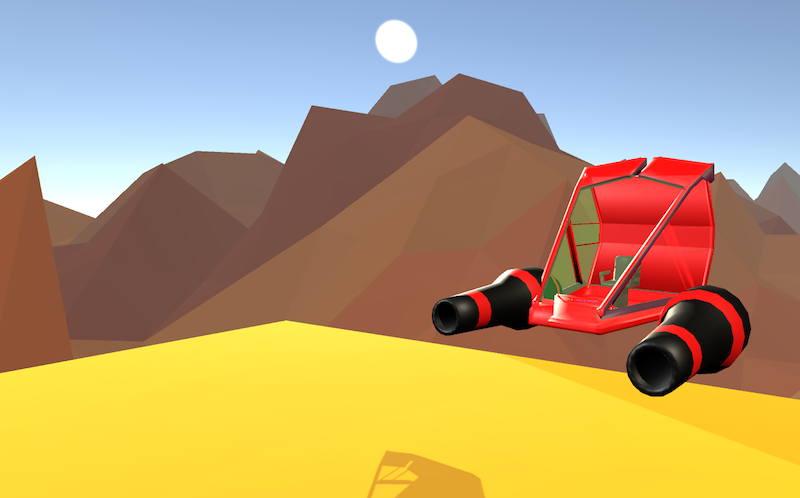
\includegraphics[scale=0.53]{images/ship.png}
\end{figure}

\begin{figure}[h]
   \caption{\label{étiquette} View from the cockpit}
   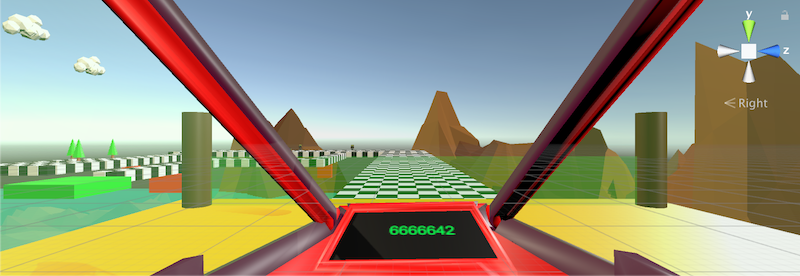
\includegraphics[scale=1]{images/cockpit.png}
\end{figure}

\section{Unity Specifics}

Here we want to mention some key unity implementation that are worth mentioning.

We used the OpenVR plugin to integrate the HMD into our game by dragging the SteamVR prefab and the Camera rig into the scene. Since our game is a seated experience we changed the "Tracking Space" parameter of the SteamVR prefab to "Tracking Universe Seated" and we use the following code to reset the initial position of the camera:

\begin{lstlisting}
Valve.VR.OpenVR.System.ResetSeatedZeroPose ();
Valve.VR.OpenVR.Compositor.SetTrackingSpace (
    Valve.VR.ETrackingUniverseOrigin.TrackingUniverseSeated);
\end{lstlisting}

Also the ResetCam.cs script makes the CameraRig follow the robot since it is not recommended to make the CameraRig a child of the vehicle directly.

To be able to develop the game without access to the HMD we implemented keyboard controls and we also found out how to disable the OpenVR plugin to remove errors. To do this, you simply add an empty Virtual Reality SDK "None" above OpenVR in Edit->Project Settings->Player.

We used rigidbody physic to move the robot. To achieve this we changed the max angular velocity of the robot rigidbody as well as good drag and angular drag values such that the robot doesn't have too much inertia but still feels like a vehicle. Then to move the robot we add relative forces and torque.

We also made a set of prefabs to ease the development of levels. That way we can instantly set up a new level simply by importing the "LevelSetup" prefab and a vehicle and all the VR code is directly in the scene. The game could easily be expanded with more levels in that manner.


\section{Discussion}

We didn't have time to recrute subject and conduct a proper trial. But we tested our game on several types of persons including men and women, skilled in computer science or not and gamer or not.

None of them reported unpleasant feelings nor motion-sickness. However, non-gamers subjects struggled to get the intuition of the controls with the Vive controllers. The notion of pitch, yaw and roll is indeed only known to gamers, game developers and in the aviation industry.

\section{Conclusion}

We learnt a lot by practicing virtual reality with this project. We are now especially skilled in projections, quaternions and spatial representation.

We did not expect to spend so much time on what we thought were basic features, but the learning curve was quite steep. We then had to reduce the number of features.

\section{Ressources}

The video providing an overview of our game is available on YouTube at this address : \href{https://www.youtube.com/watch?v=8nC1i0AayuY}{www.youtube.com/watch?v=8nC1i0AayuY}. Feel free to share it broadly and use it as you want.

The codebase is entirely available on GitHub at this address : \href{https://github.com/Ahaeflig/VR6}{www.github.com/Ahaeflig/VR6}. We encourage you to submit issues and/or pull requests on the project if you want to collaborate and participate to the development of the game.


\end{document}